\section{Zahlenmengen}

\hfill \break
Wichtige Symbole;
\begin{itemize}
    \item nur positive Zahlen und Null:  $\mathbb{Z}_0^{+}$
    \item nur negative Zahlen und Null: $\mathbb{Z}_0^{-}$
    \item nur positive Zahlen: $\mathbb{Z}^{+}$
    \item nur negative Zahlen: $\mathbb{Z}^{-}$
    \item Element von: $11-15 = -4 \in \mathbb{Z}$
    \item kein Element von: $11-15 = -4 \notin \mathbb{N}$
\end{itemize}

Diagramm der Zahlenmengen:\\
\hfill \break
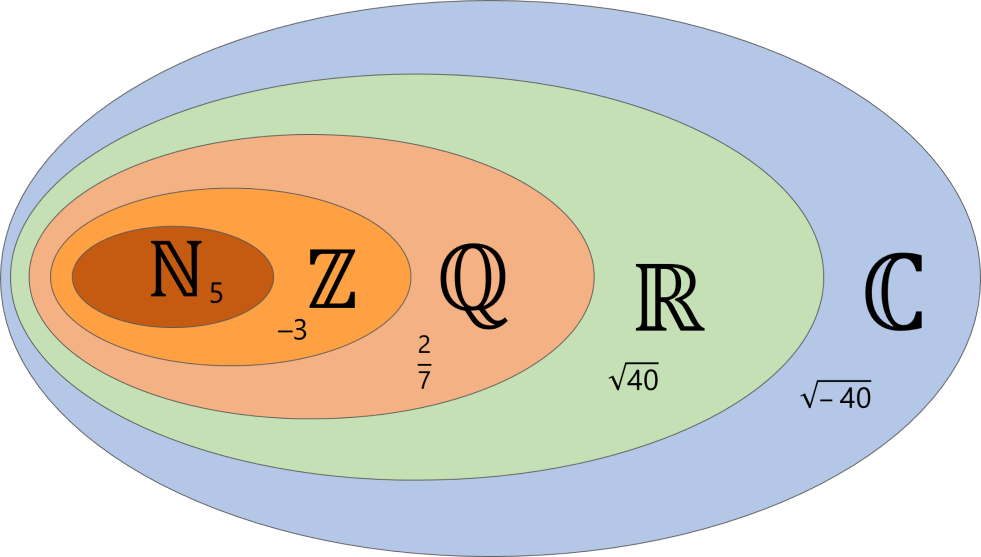
\includegraphics[scale=0.4]{Zahlenmengen}

\break
\input{Topics/Zahlenmengen/SubTopics/NatürlichenZahlen}
\break
\subsection{Die Ganzen Zahlen}
Symbol: $\mathbb{Z}$\\
sind alle Ganzen Zahlen Positiv als auch Negatiev

\hfill \break
\hfill \break
$ \mathbb{Z}=\{\ldots,-3,-2,-1,0,1,2,3,\ldots\} $

\hfill \break
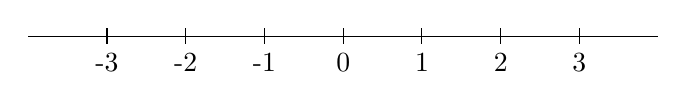
\begin{tikzpicture}
    \draw (-4,0) -- (4,0);
    \foreach \X in {-3,...,3}
    \draw (\X,0.1) -- (\X,-0.1);
    \foreach \X in {-3,-2,-1,0,1,2,3}
    \node[anchor=north] at (\X,-0.1){\X};
\end{tikzpicture}

\hfill \break
Möglichkeiten mit den Ganzen Zahlen:
\begin{enumerate}
    \item Subtrahieren ist uneingeschränkt möglich:
          \begin{itemize}
              \item 1-3 = -2
              \item 10-5 = 5
          \end{itemize}
    \item Dividieren ist nur eingeschränkt möglich:
          \begin{itemize}
              \item 1/3 = ?
              \item 10/5 = 2
          \end{itemize}
\end{enumerate}
\break
\subsection{Die Ratiaonalen Zahlen}
Symbol: $\mathbb{Q}$\\
sind die Menge aller Brüche

\hfill \break
\hfill \break
$ \mathbb{Q}=\{\frac{2}{3},\frac{7}{6},\frac{1}{6},1\frac{6}{7},0.125,0.\overline{3},\ldots\} $

\hfill \break
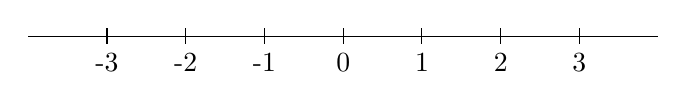
\begin{tikzpicture}
    \draw (-4,0) -- (4,0);
    \foreach \X in {-3,...,3}
    \draw (\X,0.1) -- (\X,-0.1);
    \foreach \X in {-3,-2,-1,0,1,2,3}
    \node[anchor=north] at (\X,-0.1){\X};
\end{tikzpicture}

\hfill \break
Benennung: 1/3 = $\frac{1}{3} = 0.\overline{3}$
\begin{itemize}
    \item 1 = Zähler, er zählt wie oft die Basis vorhanden ist
    \item 3 = Nenner, er gibt die Basis an
\end{itemize}

\hfill \break
Es bibt endliche und unendliche Dezimalzahlen:
\begin{itemize}
    \item endliche: 0.25
    \item unendliche: $0.\overline{25}$
\end{itemize}

\hfill \break
Möglichkeiten mit den Ganzen Zahlen:
\begin{enumerate}
    \item Dividieren ist ist uneingeschränkt möglich:
          \begin{itemize}
              \item 1/3 = $0.\overline{3}$
              \item 10/5 = 2
          \end{itemize}
\end{enumerate}

\hfill \break
Bekannte Büche:
\begin{itemize}
    \item $\frac{1}{5} = 0.2$
    \item $\frac{1}{4} = 0.25$
    \item $\frac{1}{2} = 0.5$
    \item $\frac{1}{8} = 0.125$
    \item $\frac{1}{9} = 0.\overline{1}$
    \item $\frac{1}{3} = 0.\overline{3}$
\end{itemize}
\break
\subsection{Die Reellen Zahlen}
Symbol: $\mathbb{R}$\\
sind alle Rationalen und irrationalen Zahlen

\hfill \break
Intervale beschreiben einen Zahlenbereich: $\{[1,2];[1.2,3.4]\}$


\hfill \break
\begin{tikzpicture}
    \draw (0,0) -- (4,0);
    \foreach \X in {1,...,3}
    \draw (\X,0.1) -- (\X,-0.1);
    \foreach \X in {1,3}
    \node[anchor=north] at (\X,-0.1){\X};
\end{tikzpicture}

\hfill \break
Zwischen 1 und 3 Liegen unendlich viele Zahlen


\hfill \break
Schreibweisen von Intervalen:
\begin{itemize}
    \item $[1,2]$ = Geschlossener Interval
    \item $[1,2) = [1,2[$ = Halboffener Interval
    \item $(1,2] = ]1,2]$ = Halboffener Interval
    \item $(1,2) = ]1,2[$ = Offener Interval
\end{itemize}



\hfill \break
Beschreibungen:
\begin{center}
    \begin{tabular}{ |c|c|c| }
        \hline
        Aufzählend             & Grafisch                                      & Beschreibend     \\
        A = $\{2,3,4,5\} $     & 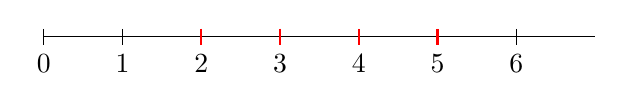
\begin{tikzpicture}
                                     \draw (0,0) -- (7,0);
                                     \foreach \X in {0,...,6}
                                     \draw (\X,0.1) -- (\X,-0.1);
                                     \foreach \X in {0,...,6}
                                     \node[anchor=north] at (\X,-0.1){\X};
                                     \foreach \X in {2,3,4,5}
                                     \draw[color=red,thick] (\X,0.1) -- (\X,-0.1);
                                 \end{tikzpicture} & A = $\{x \in \mathbb{N} | 2 \leq x \leq 5\}$ \\
        B = $\{-2,-1,0,1,2\} $ & 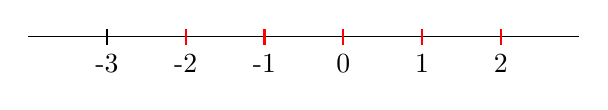
\begin{tikzpicture}
                                     \draw (-4,0) -- (3,0);
                                     \foreach \X in {-3,...,2}
                                     \draw (\X,0.1) -- (\X,-0.1);
                                     \foreach \X in {-3,...,2}
                                     \node[anchor=north] at (\X,-0.1){\X};
                                     \foreach \X in {-2,...,2}
                                     \draw[color=red,thick] (\X,0.1) -- (\X,-0.1);
                                 \end{tikzpicture} & B = $\{x \in \mathbb{Z} |-2 \leq x < 2\}$    \\
        C = $[-1,3]$           & 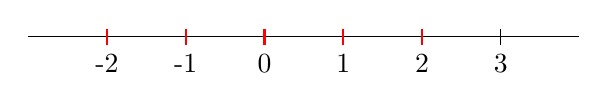
\begin{tikzpicture}
                                     \draw (-3,0) -- (4,0);
                                     \foreach \X in {-2,...,3}
                                     \draw (\X,0.1) -- (\X,-0.1);
                                     \foreach \X in {-2,...,3}
                                     \node[anchor=north] at (\X,-0.1){\X};
                                     \foreach \X in {-2,...,2}
                                     \draw[color=red,thick] (\X,0.1) -- (\X,-0.1);
                                 \end{tikzpicture} & C = $\{x \in \mathbb{R} |-1 \leq x < 3\}$    \\
        D = $]2,5]$            & 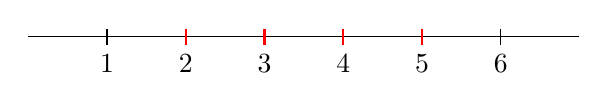
\begin{tikzpicture}
                                     \draw (0,0) -- (7,0);
                                     \foreach \X in {1,...,6}
                                     \draw (\X,0.1) -- (\X,-0.1);
                                     \foreach \X in {1,...,6}
                                     \node[anchor=north] at (\X,-0.1){\X};
                                     \foreach \X in {2,...,5}
                                     \draw[color=red,thick] (\X,0.1) -- (\X,-0.1);
                                 \end{tikzpicture} & D = $\{x \in \mathbb{R} | 2 < x \leq 5\}$    \\
        \hline
    \end{tabular}
\end{center}


